\documentclass[a4paper, 11pt]{article}
\usepackage{graphicx}
\usepackage{multicol}
\usepackage{tabularx}
\usepackage{enumitem}
\usepackage[a4paper, margin=1.8cm]{geometry}
\usepackage{listings}
\usepackage{amssymb}
\usepackage{gvv}
\usepackage{gvv-book}
\usepackage{amsmath}
\usepackage{setspace}
\usepackage{caption}
\usepackage{float}

\graphicspath{/figs}

\begin{document}
\begin{center}
    \huge{EC : ELECTRONICS AND COMMUNICATION ENGINEERING}\\
    \large{EE25BTECH11041 - Naman Kumar}
\end{center}

\begin{enumerate}
    \item The modes in a rectangular waveguide are denoted by $TE_{mn}/TM_{mn}$ where m and n are the eigen numbers along the larger and smaller dimensions of the waveguide respectively. Which one of the following statements is TRUE?
    
    \begin{enumerate}
        \item The $TM_{10}$ mode of the waveguide does not exist
        \item The $TE_{10}$ mode of the waveguide does not exist
        \item The $TM_{10}$ and the $TE_{10}$ modes both exist and have the same cut-off frequencies
        \item The $TM_{10}$ and the $TM_{01}$ modes both exist and have the same cut-off frequencies
    \end{enumerate}

    \hfill{\brak{\text{GATE EC 2011}}}

    \item The Column-1 lists the attributes and the Column-2 lists the modulation systems. Match the attribute to the modulation system that best meets it.
    
    \begin{table}[H]
        \centering
        \begin{tabular}{ll}
            \textbf{Column-1} & \textbf{Column-2} \\
            P. Power efficient transmission of signals & I. Conventional AM \\
            Q. Most bandwidth efficient transmission of voice signals & II. FM \\
            R. Simplest receiver structure & III. VSB \\
            S. Bandwidth efficient transmission of signals with & IV. SSB-SC \\
            \quad significant dc component & \\
        \end{tabular}
        \caption*{}
        \label{tab:q2}
    \end{table}
    
    \begin{enumerate}
        \begin{multicols}{2}
            \item P-IV, Q-II, R-I, S-III
            \item P-II, Q-IV, R-I, S-III
            \item P-III, Q-II, R-I, S-IV
            \item P-II, Q-IV, R-III, S-I
        \end{multicols}
    \end{enumerate}

    \hfill{\brak{\text{GATE EC 2011}}}

    \item The differential equation $100\frac{d^{2}y}{dt^{2}}-20\frac{dy}{dt}+y=x\brak{t}$ describes a system with an input $x\brak{t}$ and an output $y\brak{t}$. The system, which is initially relaxed, is excited by a unit step input. The output $y\brak{t}$ can be represented by the waveform
    
    \begin{enumerate}
        \item \begin{figure}[H] \centering \includegraphics[width=0.4\columnwidth]{figs/q3A.png} \caption*{} \label{fig:a3A} \end{figure}
        \item \begin{figure}[H] \centering \includegraphics[width=0.4\columnwidth]{figs/q3B.png} \caption*{} \label{fig:a3B} \end{figure}
        \item \begin{figure}[H] \centering \includegraphics[width=0.4\columnwidth]{figs/q3C.png} \caption*{} \label{fig:a3C} \end{figure}
        \item \begin{figure}[H] \centering \includegraphics[width=0.4\columnwidth]{figs/q3D.png} \caption*{} \label{fig:a3D} \end{figure}
    \end{enumerate}

    \hfill{\brak{\text{GATE EC 2011}}}

    \item For the transfer function $G\brak{j\omega}=5+j\omega$ the corresponding Nyquist plot for positive frequency has the form
    \begin{enumerate}
        \item \begin{figure}[H] \centering \includegraphics[width=0.3\columnwidth]{figs/q4A.png} \caption*{} \label{fig:a4A} \end{figure}
        \item \begin{figure}[H] \centering \includegraphics[width=0.3\columnwidth]{figs/q4B.png} \caption*{} \label{fig:a4B} \end{figure}
        \item \begin{figure}[H] \centering \includegraphics[width=0.3\columnwidth]{figs/q4C.png} \caption*{} \label{fig:a4C} \end{figure}
        \item \begin{figure}[H] \centering \includegraphics[width=0.3\columnwidth]{figs/q4D.png} \caption*{} \label{fig:a4D} \end{figure}
    \end{enumerate}

    \hfill{\brak{\text{GATE EC 2011}}}

    \item The trigonometric Fourier series of an even function does not have the
    
    \begin{enumerate}
        \begin{multicols}{2}
            \item dc term
            \item cosine terms
            \item sine terms
            \item odd harmonic terms
        \end{multicols}
    \end{enumerate}

    \hfill{\brak{\text{GATE EC 2011}}}

    \item When the output Y in the circuit below is "1", it implies that data has
    
    \begin{figure}[H]
        \centering
        \includegraphics[width=0.7\columnwidth]{figs/q6.png}
        \caption*{}
        \label{fig:q6}
    \end{figure}
    
    \begin{enumerate}
        \item changed from "0" to "1"
        \item changed from "1" to "0"
        \item changed in either direction
        \item not changed
    \end{enumerate}

    \hfill{\brak{\text{GATE EC 2011}}}

    \item The logic function implemented by the circuit below is \brak{\text{ground implies a logic "0"}}
    
    \begin{figure}[H]
        \centering
        \includegraphics[width=0.6\columnwidth]{figs/q7.png}
        \caption*{}
        \label{fig:q7}
    \end{figure}
    
    \begin{enumerate}
        \begin{multicols}{2}
            \item $F = \text{AND}\brak{P,Q}$
            \item $F = \text{OR}\brak{P,Q}$
            \item $F = \text{XNOR}\brak{P,Q}$
            \item $F = \text{XOR}\brak{P,Q}$
        \end{multicols}
    \end{enumerate}

    \hfill{\brak{\text{GATE EC 2011}}}

    \item The circuit below implements a filter between the input current $i_{i}$ and the output voltage $v_{0}$. Assume that the opamp is ideal. The filter implemented is a
    
    \begin{figure}[H]
        \centering
        \includegraphics[width=0.6\columnwidth]{figs/q8.png}
        \caption*{}
        \label{fig:q8}
    \end{figure}
    
    \begin{enumerate}
        \begin{multicols}{2}
            \item low pass filter
            \item band pass filter
            \item band stop filter
            \item high pass filter
        \end{multicols}
    \end{enumerate}

    \hfill{\brak{\text{GATE EC 2011}}}

    \item A silicon PN junction is forward biased with a constant current at room temperature. When the temperature is increased by $10\degree$C, the forward bias voltage across the PN junction
    
    \begin{enumerate}
        \begin{multicols}{2}
            \item increases by $60$ mV
            \item decreases by $60$ mV
            \item increases by $25$ mV
            \item decreases by $25$ mV
        \end{multicols}
    \end{enumerate}

    \hfill{\brak{\text{GATE EC 2011}}}

    \item In the circuit shown below, the Norton equivalent current in amperes with respect to the terminals P and Q is
    
    \begin{figure}[H]
        \centering
        \includegraphics[width=0.5\columnwidth]{figs/q10.png}
        \caption*{}
        \label{fig:q10}
    \end{figure}
    
    \begin{enumerate}
        \begin{multicols}{2}
            \item $6.4-j4.8$
            \item $6.56-j7.87$
            \item $10+j0$
            \item $16+j0$
        \end{multicols}
    \end{enumerate}

    \hfill{\brak{\text{GATE EC 2011}}}

    \item In the circuit shown below, the value of $R_{L}$ such that the power transferred to $R_{L}$ is maximum is
    
    \begin{figure}[H]
        \centering
        \includegraphics[width=0.7\columnwidth]{figs/q11.png}
        \caption*{}
        \label{fig:q11}
    \end{figure}
    
    \begin{enumerate}
        \begin{multicols}{4}
            \item $5$ \ohm
            \item $10$ \ohm
            \item $15$ \ohm
            \item $20$ \ohm
        \end{multicols}
    \end{enumerate}

    \hfill{\brak{\text{GATE EC 2011}}}

    \item The value of the integral $\oint_{C}\frac{-3z+4}{\brak{z^{2}+4z+5}}dz$ where c is the circle $\abs{z}=1$ is given by
    
    \begin{enumerate}
        \begin{multicols}{4}
            \item $0$
            \item $1/10$
            \item $4/5$
            \item $1$
        \end{multicols}
    \end{enumerate}

    \hfill{\brak{\text{GATE EC 2011}}}

    \item A transmission line of characteristic impedance $50$ \ohm is terminated by a $50$ \ohm load. When excited by a sinusoidal voltage source at $10$ GHz, the phase difference between two points spaced $2$ mm apart on the line is found to be $\pi/4$ radians. The phase velocity of the wave along the line is
    
    \begin{enumerate}
        \begin{multicols}{2}
            \item $0.8 \times 10^{8}$ m/s
            \item $1.2 \times 10^{8}$ m/s
            \item $1.6 \times 10^{8}$ m/s
            \item $3 \times 10^{8}$ m/s
        \end{multicols}
    \end{enumerate}

    \hfill{\brak{\text{GATE EC 2011}}}

    \item Consider the following statements regarding the complex Poynting vector $\vec{P}$ for the power radiated by a point source in an infinite homogeneous and lossless medium. $\text{Re}\brak{\vec{P}}$ denotes the real part of $\vec{P}$, S denotes a spherical surface whose centre is at the point source, and $\hat{n}$ denotes the unit surface normal on S. Which of the following statements is TRUE?
    
    \begin{enumerate}
        \item $\text{Re}\brak{\vec{P}}$ remains constant at any radial distance from the source
        \item $\text{Re}\brak{\vec{P}}$ increases with increasing radial distance from the source
        \item $\oint\oint_{S}\text{Re}\brak{\vec{P}} \cdot \hat{n} dS$ remains constant at any radial distance from the source
        \item $\oint\oint_{S}\text{Re}\brak{\vec{P}} \cdot \hat{n} dS$ decreases with increasing radial distance from the source
    \end{enumerate}

    \hfill{\brak{\text{GATE EC 2011}}}

    \item An analog signal is band-limited to $4$ kHz, sampled at the Nyquist rate and the samples are quantized into $4$ levels. The quantized levels are assumed to be independent and equally probable. If we transmit two quantized samples per second, the information rate is
    
    \begin{enumerate}
        \begin{multicols}{4}
            \item $1$ bit/sec
            \item $2$ bits/sec
            \item $3$ bits/sec
            \item $4$ bits/sec
        \end{multicols}
    \end{enumerate}
    
    \hfill{\brak{\text{GATE EC 2011}}}

    \item The root locus plot for a system is given below. The open loop transfer function corresponding to this plot is given by
    
    \begin{figure}[H]
        \centering
        \includegraphics[width=0.6\columnwidth]{figs/q16.png}
        \caption*{}
        \label{fig:q16}
    \end{figure}
    
    \begin{enumerate}
    \begin{multicols}{2}
        \item $G\brak{s}H\brak{s}=k\frac{s\brak{s+1}}{\brak{s+2}\brak{s+3}}$
        \item $G\brak{s}H\brak{s}=k\frac{\brak{s+1}}{s\brak{s+2}\brak{s+3}^{2}}$
        \item $G\brak{s}H\brak{s}=k\frac{1}{s\brak{s-1}\brak{s+2}\brak{s+3}}$
        \item $G\brak{s}H\brak{s}=k\frac{\brak{s+1}}{s\brak{s+2}\brak{s+3}}$
    \end{multicols}
    \end{enumerate}

    \hfill{\brak{\text{GATE EC 2011}}}
    \item A system is defined by its impulse response $h\brak{n}=2^{n}u\brak{n-2}$. The system is
    
    \begin{enumerate}
        \begin{multicols}{2}
            \item stable and causal
            \item causal but not stable
            \item stable but not causal
            \item unstable and noncausal
        \end{multicols}
    \end{enumerate}

    \hfill{\brak{\text{GATE EC 2011}}}

    \item If the unit step response of a network is $\brak{1-e^{-\alpha t}}$, then its unit impulse response is
    
    \begin{enumerate}
        \begin{multicols}{4}
            \item $\alpha e^{-\alpha t}$
            \item $\alpha^{-1}e^{-\alpha t}$
            \item $\brak{1-\alpha^{-1}}e^{-\alpha t}$
            \item $\brak{1-\alpha}e^{-\alpha t}$
        \end{multicols}
    \end{enumerate}

    \hfill{\brak{\text{GATE EC 2011}}}

    \item The output Y in the circuit below is always "1" when
    
    \begin{figure}[H]
        \centering
        \includegraphics[width=0.7\columnwidth]{figs/q19.png}
        \caption*{}
        \label{fig:q19}
    \end{figure}
    
    \begin{enumerate}
        \item two or more of the inputs P, Q, R are "0"
        \item two or more of the inputs P, Q, R are "1"
        \item any odd number of the inputs P, Q, R is "0"
        \item any odd number of the inputs P, Q, R is "1"
    \end{enumerate}

    \hfill{\brak{\text{GATE EC 2011}}}

    \item In the circuit shown below, capacitors $C_{1}$ and $C_{2}$ are very large and are shorts at the input frequency. $v_{i}$ is a small signal input. The gain magnitude $\abs{v_{o}/v_{i}}$ at $10$ Mrad/s is
    
    \begin{figure}[H]
        \centering
        \includegraphics[width=0.5\columnwidth]{figs/q20.png}
        \caption*{}
        \label{fig:q20}
    \end{figure}
    
    \begin{enumerate}
        \begin{multicols}{2}
            \item maximum
            \item minimum
            \item unity
            \item zero
        \end{multicols}
    \end{enumerate}

    \hfill{\brak{\text{GATE EC 2011}}}

    \item Drift current in semiconductors depends upon
    
    \begin{enumerate}
        \item only the electric field
        \item only the carrier concentration gradient
        \item both the electric field and the carrier concentration
        \item both the electric field and the carrier concentration gradient
    \end{enumerate}

    \hfill{\brak{\text{GATE EC 2011}}}

    \item A Zener diode, when used in voltage stabilization circuits, is biased in
    
    \begin{enumerate}
        \item reverse bias region below the breakdown voltage
        \item reverse breakdown region
        \item forward bias region
        \item forward bias constant current mode
    \end{enumerate}

    \hfill{\brak{\text{GATE EC 2011}}}

    \item The circuit shown below is driven by a sinusoidal input $v_{i}=V_{p}\cos\brak{t/RC}$. The steady state output $v_{0}$ is
    
    \begin{figure}[H]
        \centering
        \includegraphics[width=0.6\columnwidth]{figs/q23.png}
        \caption*{}
        \label{fig:q23}
    \end{figure}
    
    \begin{enumerate}
        \begin{multicols}{2}
            \item $\brak{V_{p}/3}\cos\brak{t/RC}$
            \item $\brak{V_{p}/3}\sin\brak{t/RC}$
            \item $\brak{V_{p}/2}\cos\brak{t/RC}$
            \item $\brak{V_{p}/2}\sin\brak{t/RC}$
        \end{multicols}
    \end{enumerate}

    \hfill{\brak{\text{GATE EC 2011}}}

    \item Consider a closed surface S surrounding a volume V. If $\vec{r}$ is the position vector of a point inside S, with $\hat{n}$ the unit normal on S, the value of the integral $\iint_{S}5\vec{r}\cdot\hat{n}dS$ is
    
    \begin{enumerate}
        \begin{multicols}{4}
            \item 3V
            \item 5V
            \item 10V
            \item 15V
        \end{multicols}
    \end{enumerate}

    \hfill{\brak{\text{GATE EC 2011}}}

    \item The solution of the differential equation $\frac{dy}{dx}=ky$, $y\brak{0}=c$ is
    
    \begin{enumerate}
        \begin{multicols}{2}
            \item $x=ce^{-ky}$
            \item $x=ke^{cy}$
            \item $y=ce^{kx}$
            \item $y=ce^{-kx}$
        \end{multicols}
    \end{enumerate}

    \hfill{\brak{\text{GATE EC 2011}}}
    
    \item The electric and magnetic fields for a TEM wave of frequency $14$ GHz in a homogeneous medium of relative permittivity $\epsilon_{r}$ and relative permeability $\mu_{r}=1$ are given by
    \begin{align*}
        \vec{E} &= E_{p}e^{j\brak{\omega t-280\pi y}}\hat{u}_{z} \text{ V/m} \\
        \vec{H} &= 3e^{j\brak{\omega t-280\pi y}}\hat{u}_{x} \text{ A/m}
    \end{align*}
    Assuming the speed of light in free space to be $3\times10^{8}$ m/s, the intrinsic impedance of free space to be $120\pi \ohm$, the relative permittivity $\epsilon_{r}$ of the medium and the electric field amplitude $E_{p}$ are
    
    \begin{enumerate}
        \begin{multicols}{2}
            \item $\epsilon_{r}=3$, $E_{p}=120\pi$
            \item $\epsilon_{r}=3$, $E_{p}=360\pi$
            \item $\epsilon_{r}=9$, $E_{p}=360\pi$
            \item $\epsilon_{r}=9$, $E_{p}=120\pi$
        \end{multicols}
    \end{enumerate}

    \hfill{\brak{\text{GATE EC 2011}}}

    \item A message signal $m\brak{t}=\cos{2000\pi t}+4\cos{4000\pi t}$ modulates the carrier $c\brak{t}=\cos{2\pi f_{c}t}$ where $f_{c}=1$ MHz to produce an AM signal. For demodulating the generated AM signal using an envelope detector, the time constant RC of the detector circuit should satisfy
    
    \begin{enumerate}
        \item $0.5 \text{ ms} < RC < 1 \text{ ms}$
        \item $1 \text{ }\mu\text{s} \ll RC < 0.5 \text{ ms}$
        \item $RC \ll 1 \text{ }\mu\text{s}$
        \item $RC \gg 0.5 \text{ ms}$
    \end{enumerate}

    \hfill{\brak{\text{GATE EC 2011}}}

    \item The block diagram of a system with one input u and two outputs $y_{1}$ and $y_{2}$ is given below.
    
    \begin{figure}[H]
        \centering
        \includegraphics[width=0.4\columnwidth]{figs/q28.png}
        \caption*{}
        \label{fig:q28}
    \end{figure}
    
    A state space model of the above system in terms of the state vector $\underline{x}$ and the output vector $\underline{y}=\sbrak{y_{1} & y_{2}}^{T}$ is
    
    \begin{enumerate}
        \item $\dot{\underline{x}}=[2]\underline{x}+[1]u; \quad \underline{y}=[\underline{1} \quad 2]\underline{x}$
        \item $\dot{\underline{x}}=[-2]\underline{x}+[1]u; \quad \underline{y}=\myvec{1 \\ 2}\underline{x}$
        \item $\dot{\underline{x}}=\myvec{-2 & 0 \\ 0 & -2}\underline{x}+\myvec{1 \\ 1}u; \quad \underline{y}=[\underline{1} \quad 2]\underline{x}$
        \item $\dot{\underline{x}}=\myvec{2 & 0 \\ 0 & 2}\underline{x}+\myvec{1 \\ 1}u; \quad \underline{y}=\myvec{1 \\ 2}\underline{x}$
    \end{enumerate}

    \hfill{\brak{\text{GATE EC 2011}}}

    \item Two systems $H_{1}\brak{z}$ and $H_{2}\brak{z}$ are connected in cascade as shown below. The overall output $y\brak{n}$ is the same as the input $x\brak{n}$ with a one unit delay. The transfer function of the second system $H_{2}\brak{z}$ is
    
    \begin{figure}[H]
        \centering
        \includegraphics[width=0.8\columnwidth]{figs/q29.png}
        \caption*{}
        \label{fig:q29}
    \end{figure}
    
    \begin{enumerate}
        \begin{multicols}{2}
            \item $\frac{\brak{1-0.6z^{-1}}}{z^{-1}\brak{1-0.4z^{-1}}}$
            \item $\frac{z^{-1}\brak{1-0.6z^{-1}}}{\brak{1-0.4z^{-1}}}$
            \item $\frac{z^{-1}\brak{1-0.4z^{-1}}}{\brak{1-0.6z^{-1}}}$
            \item $\frac{\brak{1-0.4z^{-1}}}{z^{-1}\brak{1-0.6z^{-1}}}$
        \end{multicols}
    \end{enumerate}
    
    \hfill{\brak{\text{GATE EC 2011}}}

    \item An 8085 assembly language program is given below. Assume that the carry flag is initially unset. The content of the accumulator after the execution of the program is
    
    \begin{lstlisting}
MVI A, 07H
RLC
MOV B,A
RLC
RLC
ADD B
RRC
    \end{lstlisting}
    
    \begin{enumerate}
        \begin{multicols}{4}
            \item 8CH
            \item 64H
            \item 23H
            \item 15H
        \end{multicols}
    \end{enumerate}

    \hfill{\brak{\text{GATE EC 2011}}}

    \item The first six points of the 8-point DFT of a real valued sequence are 5, 1-j3, 0, 3-j4, 0 and 3+j4. The last two points of the DFT are respectively
    
    \begin{enumerate}
        \begin{multicols}{2}
            \item 0, 1-j3
            \item 0, 1+j3
            \item 1+j3, 5
            \item 1-j3, 5
        \end{multicols}
    \end{enumerate}
    
    \hfill{\brak{\text{GATE EC 2011}}}

    \item For the BJT $Q_{1}$ in the circuit shown below, $\beta=\infty, V_{BEon}=0.7V, V_{CEsat}=0.7V$. The switch is initially closed. At time $t=0$, the switch is opened. The time t at which $Q_{1}$ leaves the active region is
    
    \begin{figure}[H]
        \centering
        \includegraphics[width=0.4\columnwidth]{figs/q32.png}
        \caption*{}
        \label{fig:q32}
    \end{figure}
    
    \begin{enumerate}
        \begin{multicols}{4}
            \item 10 ms
            \item 25 ms
            \item 50 ms
            \item 100 ms
        \end{multicols}
    \end{enumerate}
    
    \hfill{\brak{\text{GATE EC 2011}}}

    \item In the circuit shown below, the network N is described by the following Y matrix: $Y=\myvec{0.1 S & -0.01 S \\ 0.01 S & 0.1S}$. The voltage gain $\frac{V_{2}}{V_{1}}$ is
    
    \begin{figure}[H]
        \centering
        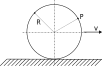
\includegraphics[width=0.7\columnwidth]{figs/q33.png}
        \caption*{}
        \label{fig:q33}
    \end{figure}
    
    \begin{enumerate}
        \begin{multicols}{4}
            \item 1/90
            \item -1/90
            \item -1/99
            \item -1/11
        \end{multicols}
    \end{enumerate}

    \hfill{\brak{\text{GATE EC 2011}}}

    \item In the circuit shown below, the initial charge on the capacitor is 2.5 mC, with the voltage polarity as indicated. The switch is closed at time $t=0$. The current $i\brak{t}$ at a time t after the switch is closed is
    
    \begin{figure}[H]
        \centering
        \includegraphics[width=0.4\columnwidth]{figs/q34.png}
        \caption*{}
        \label{fig:q34}
    \end{figure}
    
    \begin{enumerate}
    \begin{multicols}{2}
        \item $i\brak{t}=15 \exp\brak{-2 \times 10^{3}t}$ A
        \item $i\brak{t}=5 \exp\brak{-2 \times 10^{3}t}$ A
        \item $i\brak{t}=10 \exp\brak{-2 \times 10^{3}t}$ A
        \item $i\brak{t}=-5 \exp\brak{-2 \times 10^{3}t}$ A
    \end{multicols}
    \end{enumerate}
    
    \hfill{\brak{\text{GATE EC 2011}}}

    \item The system of equations
    \begin{align*}
        x+y+z &= 6 \\
        x+4y+6z &= 20 \\
        x+4y+\lambda z &= \mu
    \end{align*}
    has NO solution for values of $\lambda$ and $\mu$ given by
    
    \begin{enumerate}
        \begin{multicols}{2}
            \item $\lambda=6, \mu=20$
            \item $\lambda=6, \mu \ne 20$
            \item $\lambda \ne 6, \mu=20$
            \item $\lambda \ne 6, \mu \ne 20$
        \end{multicols}
    \end{enumerate}

    \hfill{\brak{\text{GATE EC 2011}}}

    \item A fair dice is tossed two times. The probability that the second toss results in a value that is higher than the first toss is
    
    \begin{enumerate}
        \begin{multicols}{4}
            \item 2/36
            \item 2/6
            \item 5/12
            \item 1/2
        \end{multicols}
    \end{enumerate}

    \hfill{\brak{\text{GATE EC 2011}}}

    \item A current sheet $\vec{J}=10\hat{u}_{y} \text{ A/m}$ lies on the dielectric interface $x=0$ between two dielectric media with $\epsilon_{r1}=5, \mu_{r1}=1$ in Region-1 $\brak{x<0}$ and $\epsilon_{r2}=2, \mu_{r2}=2$ in Region-2 $\brak{x>0}$. If the magnetic field in Region-1 at $x=0^{-}$ is $\vec{H}_{1}=3\hat{u}_{x}+30\hat{u}_{y} \text{ A/m}$, the magnetic field in Region-2 at $x=0^{+}$ is
    
    \begin{figure}[H]
        \centering
        \includegraphics[width=0.6\columnwidth]{figs/q37.png}
        \caption*{}
        \label{fig:q37}
    \end{figure}
    
    \begin{enumerate}
        \item $\vec{H}_{2}=1.5\hat{u}_{x}+30\hat{u}_{y}-10\hat{u}_{z} \text{ A/m}$
        \item $\vec{H}_{2}=3\hat{u}_{x}+30\hat{u}_{y}-10\hat{u}_{z} \text{ A/m}$
        \item $\vec{H}_{2}=1.5\hat{u}_{x}+40\hat{u}_{y} \text{ A/m}$
        \item $\vec{H}_{2}=3\hat{u}_{x}+30\hat{u}_{y}+10\hat{u}_{z} \text{ A/m}$
    \end{enumerate}
    
    \hfill{\brak{\text{GATE EC 2011}}}
    \item A transmission line of characteristic impedance 50 \ohm is terminated in a load impedance $Z_{L}$. The VSWR of the line is measured as 5 and the first of the voltage maxima in the line is observed at a distance of $\lambda/4$ from the load. The value of $Z_{L}$ is
    
    \begin{enumerate}
        \begin{multicols}{2}
            \item 10 \ohm
            \item 250 \ohm
            \item $\brak{19.23+j46.15}\ohm$
            \item $\brak{19.23-j46.15}\ohm$
        \end{multicols}
    \end{enumerate}

    \hfill{\brak{\text{GATE EC 2011}}}

    \item $X\brak{t}$ is a stationary random process with autocorrelation function $R_{x}\brak{\tau}=\exp\brak{-\pi\tau^{2}}$. This process is passed through the system shown below. The power spectral density of the output process $Y\brak{t}$ is
    
    \begin{figure}[H]
        \centering
        \includegraphics[width=0.7\columnwidth]{figs/q39.png}
        \caption*{}
        \label{fig:q39}
    \end{figure}
    
    \begin{enumerate}
        \item $\brak{4\pi^{2}f^{2}+1}\exp\brak{-\pi f^{2}}$
        \item $\brak{4\pi^{2}f^{2}-1}\exp\brak{-\pi f^{2}}$
        \item $\brak{4\pi^{2}f^{2}+1}\exp\brak{-\pi f}$
        \item $\brak{4\pi^{2}f^{2}-1}\exp\brak{-\pi f}$
    \end{enumerate}

    \hfill{\brak{\text{GATE EC 2011}}}

    \item The output of a 3-stage Johnson (twisted-ring) counter is fed to a digital-to-analog (D/A) converter as shown in the figure below. Assume all states of the counter to be unset initially. The waveform which represents the D/A converter output $V_{o}$ is
    
    \begin{figure}[H]
        \centering
        \includegraphics[width=0.5\columnwidth]{figs/q40.png}
        \caption*{}
        \label{fig:q40}
    \end{figure}
    
    \begin{enumerate}
        \item \begin{figure}[H]\centering\includegraphics[width=0.45\columnwidth]{figs/q40A.png}\caption*{}\label{fig:a40A}\end{figure}
        \item \begin{figure}[H]\centering\includegraphics[width=0.45\columnwidth]{figs/q40B.png}\caption*{}\label{fig:a40B}\end{figure}
        \item \begin{figure}[H]\centering\includegraphics[width=0.45\columnwidth]{figs/q40C.png}\caption*{}\label{fig:a40C}\end{figure}
        \item \begin{figure}[H]\centering\includegraphics[width=0.45\columnwidth]{figs/q40D.png}\caption*{}\label{fig:a40D}\end{figure}
    \end{enumerate}

    \hfill{\brak{\text{GATE EC 2011}}}

    \item Two D flip-flops are connected as a synchronous counter that goes through the following $Q_{B}Q_{A}$ sequence $00 \rightarrow 11 \rightarrow 01 \rightarrow 10 \rightarrow 00 \rightarrow \dots$
    The connections to the inputs $D_{A}$ and $D_{B}$ are
    
    \begin{enumerate}
        \item $D_{A}=Q_{B}, D_{B}=Q_{A}$
        \item $D_{A}=\overline{Q}_{A}, D_{B}=\overline{Q}_{B}$
        \item $D_{A}=\brak{Q_{A}\overline{Q}_{B}+\overline{Q}_{A}Q_{B}}, D_{B}=Q_{A}$
        \item $D_{A}=\brak{Q_{A}Q_{B}+\overline{Q}_{A}\overline{Q}_{B}}, D_{B}=\overline{Q}_{B}$
    \end{enumerate}

    \hfill{\brak{\text{GATE EC 2011}}}

    \item In the circuit shown below, for the MOS transistors, $\mu_{n}C_{ox}=100 \mu A/V^{2}$ and the threshold voltage $V_{T}=1$ V. The voltage $V_{x}$ at the source of the upper transistor is
    
    \begin{figure}[H]
        \centering
        \includegraphics[width=0.2\columnwidth]{figs/q42.png}
        \caption*{}
        \label{fig:q42}
    \end{figure}
    
    \begin{enumerate}
        \begin{multicols}{4}
            \item 1 V
            \item 2 V
            \item 3 V
            \item 3.67 V
        \end{multicols}
    \end{enumerate}

    \hfill{\brak{\text{GATE EC 2011}}}

    \item An input $x\brak{t}=\exp\brak{-2t}u\brak{t}+\delta\brak{t-6}$ is applied to an LTI system with impulse response $h\brak{t}=u\brak{t}$. The output is
    
    \begin{enumerate}
    \begin{multicols}{2}
        \item $[1-\exp\brak{-2t}]u\brak{t}+u\brak{t+6}$
        \item $[1-\exp\brak{-2t}]u\brak{t}+u\brak{t-6}$
        \item $0.5[1-\exp\brak{-2t}]u\brak{t}+u\brak{t+6}$
        \item $0.5[1-\exp\brak{-2t}]u\brak{t}+u\brak{t-6}$
    \end{multicols}
    \end{enumerate}

    \hfill{\brak{\text{GATE EC 2011}}}

    \item For a BJT, the common-base current gain $\alpha=0.98$ and the collector base junction reverse bias saturation current $I_{CO}=0.6 \mu A$. This BJT is connected in the common emitter mode and operated in the active region with a base drive current $I_{B}=20 \mu A$. The collector current $I_{C}$ for this mode of operation is
    
    \begin{enumerate}
        \begin{multicols}{4}
            \item 0.98 mA
            \item 0.99 mA
            \item 1.0 mA
            \item 1.01 mA
        \end{multicols}
    \end{enumerate}

    \hfill{\brak{\text{GATE EC 2011}}}

    \item If $F\brak{s}=L[f\brak{t}]=\frac{2\brak{s+1}}{s^{2}+4s+7}$ then the initial and final values of $f\brak{t}$ are respectively
    
    \begin{enumerate}
        \begin{multicols}{4}
            \item 0, 2
            \item 2, 0
            \item 0, 2/7
            \item 2/7, 0
        \end{multicols}
    \end{enumerate}
    
    \hfill{\brak{\text{GATE EC 2011}}}

    \item In the circuit shown below, the current I is equal to
    
    \begin{figure}[H]
        \centering
        \includegraphics[width=0.4\columnwidth]{figs/q46.png}
        \caption*{}
        \label{fig:q46}
    \end{figure}
    
    \begin{enumerate}
        \begin{multicols}{4}
            \item $1.4\angle0^{\circ}$ A
            \item $2.0\angle0^{\circ}$ A
            \item $2.8\angle0^{\circ}$ A
            \item $3.2\angle0^{\circ}$ A
        \end{multicols}
    \end{enumerate}
    
    \hfill{\brak{\text{GATE EC 2011}}}

    \item A numerical solution of the equation $f\brak{x}=x+\sqrt{x}-3=0$ can be obtained using Newton-Raphson method. If the starting value is $x=2$ for the iteration, the value of x that is to be used in the next step is
    
    \begin{enumerate}
        \begin{multicols}{4}
            \item 0.306
            \item 0.739
            \item 1.694
            \item 2.306
        \end{multicols}
    \end{enumerate}
    \hfill{\brak{\text{GATE EC 2011}}}
    
    The channel resistance of an N-channel JFET shown in the figure below is 600 $\Omega$ when the full channel thickness $\brak{t_{ch}}$ of $10 \mu m$ is available for conduction. The built-in voltage of the gate $P^{+}N$ junction $\brak{V_{bi}}$ is -1 V. When the gate to source voltage $\brak{V_{GS}}$ is 0 V, the channel is depleted by $1 \mu m$ on each side due to the built-in voltage and hence the thickness available for conduction is only $8 \mu m$.
    \begin{figure}[H]
        \centering
        \includegraphics[width=0.3\columnwidth]{figs/q48_49.png}
        \caption*{}
        \label{fig:q48_49}
    \end{figure}

    \item The channel resistance when $V_{GS}=0$ V is
    \begin{enumerate}
        \begin{multicols}{4}
            \item 480 $\Omega$
            \item 600 $\Omega$
            \item 750 $\Omega$
            \item 1000 $\Omega$
        \end{multicols}
    \end{enumerate}
    
    \hfill{\brak{\text{GATE EC 2011}}}

    \item The channel resistance when $V_{GS}=-3$ V is
    \begin{enumerate}
        \begin{multicols}{4}
            \item 360 $\Omega$
            \item 917 $\Omega$
            \item 1000 $\Omega$
            \item 3000 $\Omega$
        \end{multicols}
    \end{enumerate}
    
    \hfill{\brak{\text{GATE EC 2011}}}

    The input-output transfer function of a plant $H\brak{s}=\frac{100}{s\brak{s+10}^{2}}$. The plant is placed in a unity negative feedback configuration as shown in the figure below.
    
    \begin{figure}[H]
        \centering
        \includegraphics[width=0.8\columnwidth]{figs/q50_51.png}
        \caption*{}
        \label{fig:q50_51}
    \end{figure}

    \item The signal flow graph that DOES NOT model the plant transfer function $H\brak{s}$ is
    
    \begin{enumerate}
        \item \begin{figure}[H]\centering\includegraphics[width=0.7\columnwidth]{figs/q50A.png}\caption*{}\label{fig:a50A}\end{figure}
        \item \begin{figure}[H]\centering\includegraphics[width=0.7\columnwidth]{figs/q50B.png}\caption*{}\label{fig:a50B}\end{figure}
        \item \begin{figure}[H]\centering\includegraphics[width=0.7\columnwidth]{figs/q50C.png}\caption*{}\label{fig:a50C}\end{figure}
        \item \begin{figure}[H]\centering\includegraphics[width=0.7\columnwidth]{figs/q50D.png}\caption*{}\label{fig:a50D}\end{figure}
    \end{enumerate}
    
    \hfill{\brak{\text{GATE EC 2011}}}

    \item The gain margin of the system under closed loop unity negative feedback is
    \begin{enumerate}
        \begin{multicols}{4}
            \item 0 dB
            \item 20 dB
            \item 26 dB
            \item 46 dB
        \end{multicols}
    \end{enumerate}
    
    \hfill{\brak{\text{GATE EC 2011}}}
    
    A four-phase and an eight-phase signal constellation are shown in the figure below.
    \begin{figure}[H]
        \centering
        \includegraphics[width=0.8\columnwidth]{figs/q52_53.png}
        \caption*{}
        \label{fig:q52_53}
    \end{figure}

    \item For the constraint that the minimum distance between pairs of signal points be d for both constellations, the radii $r_{1}$ and $r_{2}$ of the circles are
    \begin{enumerate}
        \item $r_{1}=0.707d, r_{2}=2.782d$
        \item $r_{1}=0.707d, r_{2}=1.932d$
        \item $r_{1}=0.707d, r_{2}=1.545d$
        \item $r_{1}=0.707d, r_{2}=1.307d$
    \end{enumerate}
    
    \hfill{\brak{\text{GATE EC 2011}}}

    \item Assuming high SNR and that all signals are equally probable, the additional average transmitted signal energy required by the 8-PSK signal to achieve the same error probability as the 4-PSK signal is
    \begin{enumerate}
        \begin{multicols}{4}
            \item 11.90 dB
            \item 8.73 dB
            \item 6.79 dB
            \item 5.33 dB
        \end{multicols}
    \end{enumerate}
    
    \hfill{\brak{\text{GATE EC 2011}}}

    In the circuit shown below, assume that the voltage drop across a forward biased diode is 0.7 V. The thermal voltage $V_{t}=kT/q=25mV$. The small signal input $v_{i}=V_{p}\cos\brak{\omega t}$ where $V_{p}=100mV$.
    
    \begin{figure}[H]
        \centering
        \includegraphics[width=0.5\columnwidth]{figs/q54_55.png}
        \caption*{}
        \label{fig:q54_55}
    \end{figure}

    \item The bias current $I_{DC}$ through the diodes is
    \begin{enumerate}
        \begin{multicols}{4}
            \item 1 mA
            \item 1.28 mA
            \item 1.5 mA
            \item 2 mA
        \end{multicols}
    \end{enumerate}
    
    \hfill{\brak{\text{GATE EC 2011}}}

    \item The ac output voltage $v_{ac}$ is
    \begin{enumerate}
        \begin{multicols}{2}
            \item $0.25 \cos\brak{\omega t}$ mV
            \item $1 \cos\brak{\omega t}$ mV
            \item $2 \cos\brak{\omega t}$ mV
            \item $22 \cos\brak{\omega t}$ mV
        \end{multicols}
    \end{enumerate}
    
    \hfill{\brak{\text{GATE EC 2011}}}

    \item The question below consists of a pair of related words followed by four pairs of words. Select the pair that best expresses the relation in the original pair: Gladiator: Arena
    
    \begin{enumerate}
        \begin{multicols}{2}
            \item dancer: stage
            \item commuter: train
            \item teacher: classroom
            \item lawyer: courtroom
        \end{multicols}
    \end{enumerate}

    \hfill{\brak{\text{GATE EC 2011}}}

    \item There are two candidates P and Q in an election. During the campaign, 40\% of the voters promised to vote for P, and rest for Q. However, on the day of election 15\% of the voters went back on their promise to vote for P and instead voted for Q. 25\% of the voters went back on their promise to vote for Q and instead voted for P. Suppose, P lost by 2 votes, then what was the total number of voters?
    
    \begin{enumerate}
        \begin{multicols}{4}
            \item 100
            \item 110
            \item 90
            \item 95
        \end{multicols}
    \end{enumerate}
    
    \hfill{\brak{\text{GATE EC 2011}}}

    \item Choose the most appropriate word from the options given below to complete the following sentence:\\It was her view that the country's problems had been \underline{\hspace{2cm}} by foreign technocrats, so that to invite them to come back would be counter-productive.
    
    \begin{enumerate}
        \begin{multicols}{2}
            \item identified
            \item ascertained
            \item exacerbated
            \item analysed
        \end{multicols}
    \end{enumerate}

    \hfill{\brak{\text{GATE EC 2011}}}

    \item Choose the word from the options given below that is most nearly opposite in meaning to the given word:
    
    Frequency
    
    \begin{enumerate}
        \begin{multicols}{2}
            \item periodicity
            \item rarity
            \item gradualness
            \item persistency
        \end{multicols}
    \end{enumerate}
    
    \hfill{\brak{\text{GATE EC 2011}}}

    \item Choose the most appropriate word from the options given below to complete the following sentence:
    
    Under ethical guidelines recently adopted by the Indian Medical Association, human genes are to be manipulated only to correct diseases for which \underline{\hspace{2cm}} treatments are unsatisfactory.
    
    \begin{enumerate}
        \begin{multicols}{2}
            \item similar
            \item most
            \item uncommon
            \item available
        \end{multicols}
    \end{enumerate}
    
    \hfill{\brak{\text{GATE EC 2011}}}

    \item The horse has played a little known but very important role in the field of medicine. Horses were injected with toxins of diseases until their blood built up immunities. Then a serum was made from their blood. Serums to fight with diphtheria and tetanus were developed this way. It can be inferred from the passage, that horses were
    
    \begin{enumerate}
        \item given immunity to diseases
        \item generally quite immune to diseases
        \item given medicines to fight toxins
        \item given diphtheria and tetanus serums
    \end{enumerate}
    
    \hfill{\brak{\text{GATE EC 2011}}}

    \item The fuel consumed by a motorcycle during a journey while traveling at various speeds is indicated in the graph below.
    
    \begin{figure}[H]
        \centering
        \includegraphics[width=0.7\columnwidth]{figs/q62.png}
        \caption*{}
        \label{fig:q62_graph}
    \end{figure}
    
    The distances covered during four laps of the journey are listed in the table below
    
    \begin{table}[H]
        \centering
        \begin{tabular}{|c|c|c|}
            \hline
            \textbf{Lap} & \textbf{Distance (kilometres)} & \textbf{Average speed (kilometres per hour)} \\
            \hline
            P & 15 & 15 \\
            Q & 75 & 45 \\
            R & 40 & 75 \\
            S & 10 & 10 \\
            \hline
        \end{tabular}
        \caption*{}
        \label{tab:q62}
    \end{table}
    
    From the given data, we can conclude that the fuel consumed per kilometre was least during the lap
    
    \begin{enumerate}
        \begin{multicols}{4}
            \item P
            \item Q
            \item R
            \item S
        \end{multicols}
    \end{enumerate}

    \hfill{\brak{\text{GATE EC 2011}}}

    \item Three friends, R, S and T shared toffee from a bowl. R took $1/3^{\text{rd}}$ of the toffees, but returned four to the bowl. S took $1/4^{\text{th}}$ of what was left but returned three toffees to the bowl. T took half of the remainder but returned two back into the bowl. If the bowl had 17 toffees left, how many toffees were originally there in the bowl?
    
    \begin{enumerate}
        \begin{multicols}{4}
            \item 38
            \item 31
            \item 48
            \item 41
        \end{multicols}
    \end{enumerate}
    
    \hfill{\brak{\text{GATE EC 2011}}}

    \item Given that $f\brak{y}=\abs{y}/y$, and q is any non-zero real number, the value of $\abs{f\brak{q}-f\brak{-q}}$ is
    
    \begin{enumerate}
        \begin{multicols}{4}
            \item 0
            \item -1
            \item 1
            \item 2
        \end{multicols}
    \end{enumerate}

    \hfill{\brak{\text{GATE EC 2011}}}

    \item The sum of n terms of the series 4+44+444+.... is
    
    \begin{enumerate}
        \item $\brak{4/81}[10^{n+1}-9n-1]$
        \item $\brak{4/81}[10^{n-1}-9n-1]$
        \item $\brak{4/81}[10^{n+1}-9n-10]$
        \item $\brak{4/81}[10^{n}-9n-10]$
    \end{enumerate}

    \hfill{\brak{\text{GATE EC 2011}}}

\end{enumerate}
\end{document}

